% -*- root: ../main.tex -*-

% Esporre lo stato di funzionamento effettivo del sistema progettato ad elaborato concluso. Per ciascuna delle funzionalità salienti devono essere tabellate e discusse le performance riscontrate mediante opportuni test eseguiti in fase di validazione del progetto. I tempi di esecuzione/comunicazione devono essere accompagnati dalle caratteristiche dell'hardware sul quale è eseguito il software. Qualora l'elaborato includa algoritmi innovativi, indicarne la complessità computazionale (avendo cura di esporre lo pseudo codice nella sezione Implementazione).
% 3000 - 6000 battute

\chapter{Testing e Performance}
\section{Automazione Gabbia e Monitoraggio Salute}
\subsection{Hardware}
Per quanto riguarda l'automazione di cibo e acqua e il monitoraggio dei parametri vitali dell'animale sono state testate multiple soluzioni hardware. In fase di validazione del progetto sono stati prese in esame principalmente due board che soddisfacessero i requisiti di economicità, connettività e prestazioni: L'ESP8266 e il successore ESP32. 
Entrambi offrono la connettività Wi-Fi integrata e buona potenza computazionale, cosa di cui è carente la board Arduino, e un costo contenuto (5€ per il primo e 7€ per il secondo, dati del primo semestre 2021) rispetto alla board Raspberry. Quest'ultima board offre connettività e prestazioni ma i costi sono decisamente fuori budget per il committente e per la natura distribuita dei compiti. La piattaforma ESP si è rivelata un buon compromesso e quindi si è passati a testarne i due differenti modelli.

Dopo i testing eseguiti in fase iniziale sono emerse differenze sostanziali nei tempi di avvio del programma e di connessione. Inoltre l'ESP8266 ha riscontrato spesso problemi nel caricamento dei file e nell'esecuzione di micropython. Di seguito si riporta la tabella riassuntiva per i tempi di esecuzione/comunicazione, accompagnati dalle caratteristiche dell'hardware. 

    \begin{figure}[H]
        \centering
        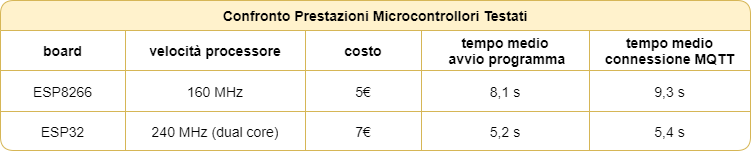
\includegraphics[width=0.9\textwidth]{DrawIo/ConfrontoMicrocontrollori.png}
    \end{figure}


Alla luce della minima differenza di prezzo tra i due device rispetto alla capacità computazionale, la scelta è ricaduta sul più recente ESP32.
\section{Videosorveglianza}
\subsection{Hardware}
Come anticipato in precedenza, il lato visione, di per se più computazionalmente oneroso, ha reso necessaria un'analisi più approfondita delle performance e la scelta è ricaduta su Raspberry Pi e ESP32-CAM. Inizialmente stato implementato un server web in C, per l'ESP ma il development è stato in seguito interrotto per la scarsa potenza potenza di quest'ultimo nell'elaborazione delle immagini. E' stato tuttavia ritenuto valido per un'alternativa economica per il semplice streaming video senza elaborazione e notifica.
Le board Raspberry Pi testate sono state le seguenti, con i rispettivi tempi di elaborazione:
    
    \begin{figure}[H]
        \centering
        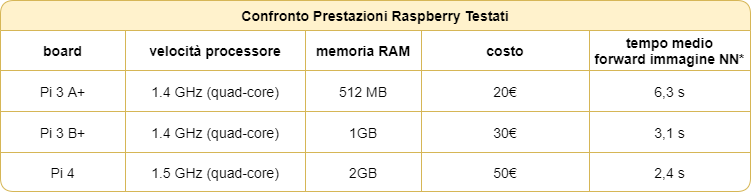
\includegraphics[width=0.9\textwidth]{DrawIo/ConfrontoRaspberry.png}
    \end{figure}

* i tempi si riferiscono all'attesa media per ottenere i risultati di object-detection attraverso una rete neurale con architettura Yolo3 con lo stesso set di immagini.

Considerando il rapporto costo/prestazioni, la scelta è ricaduta sul Raspberry Pi 3 B+ che con soli 0.7 secondi di distacco dal suo successore si posiziona su una fascia decisamente più economica.


\subsection{Software}
Per quanto riguarda il software sono state testate le prestazioni dei due metodi per la detection di anomalie/intrusioni.Il secondo, più elaborato, su riconoscimento oggetti per mezzo di una rete neurale. 
    \subsubsection{Motion Detection} Il primo, più lineare, si basa su elaborazione delle immagini tramite sottrazione dello sfondo per rilevare del movimento. Le semplici operazioni di sfocatura gaussiana, differenza, soglia e calcolo dell'area sono state studiate per ottenere alte prestazioni circa la velocità di esecuzione dell'algoritmo. 
    I test sperimentali sulla piattaforma scelta Raspberry Pi 3B+ hanno rilevato una media di 30 FPS sul materiale di test. Questa misura si è rivelata parecchio costante, poiché l'algoritmo non effettua un'analisi semantica delle immagini ma semplicemente delle operazioni matematiche indipendentemente dal contenuto. L'unico overhead dell'algoritmo risiede infatti nel calcolo dell'area dell'immagine cambiata qualora presente. Più questa è grande più tempo viene impiegato per calcolarla. Rispetto ai tempi di esecuzione e alle normale fluttuazioni delle prestazioni non è stata rilevata una differenza degna di nota (Si vedano gli FPS nonostante la grande area rilevata in [Fig. \ref{fig:MDcomparison}] 
    
    \begin{figure}[H]
        \caption{Surveillance with Motion Detection}
        \label{fig:MDcomparison}
        \centering
        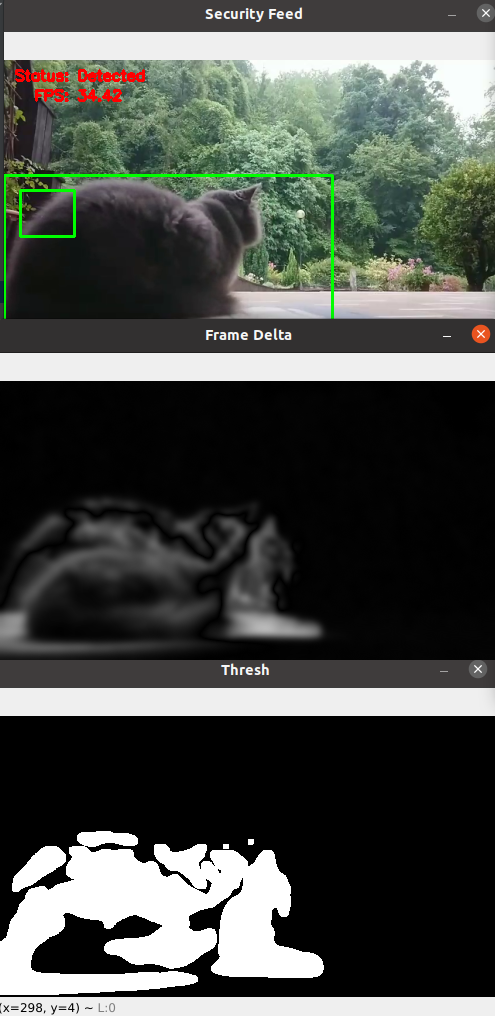
\includegraphics[width=0.5\textwidth]{Images/MDcomparison.png}
    \end{figure}
    
    La velocità dell'algoritmo va a discapito della precisione dello stesso. A seguito delle rilevazioni la matrice di confusione risulta non ottimale. Le motivazioni principali trovate risiedono nei seguenti scenari:
    \begin{itemize}
        \item qualora una figura da rilevare stesse ferma o si muovesse lentamente, la soglia non sarebbe abbastanza alta da venir rilevata e ciò comporta dei falsi negativi. Non avendo nozione della semantica dell'immagine, l'algoritmo non può venir calibrato ulteriormente.
        \item qualora un oggetto irrilevante (es: una mosca che passa vicino sulle lenti) produca un cambiamento significativo nell'immagine, la soglia viene superata e viene prodotto un falso positivo. Anche qui la mancanza di discernimento dell'algoritmo non può essere superata se non cambiandolo.
        \item qualora l'oggetto estraneo sia lontano l'area di cambiamento risulta piccola e non supera la soglia, producendo falsi negativi. Se la soglia viene abbassata si incorre in falsi positivi per via di minimi cambiamenti ambientali.
    \end{itemize}
    
    La matrice di confusione risultante in [Fig. \ref{fig:MDmatrix}] risulta chiaramente sbilanciata con parecchi falsi positivi. Questo deriva chiaramente dall'impossibilità discussa di discernere tra oggetti in movimento "non allarmanti" e viceversa.
    Per ovviare a questo problema nella sezione successiva si discuterà l'uso delle reti neurali e le prestazioni inerenti l'uso dell'object-detection.
    \begin{figure}[H]
        \caption{Confusion matrix of Motion Detection}
        \label{fig:MDmatrix}
        \centering
        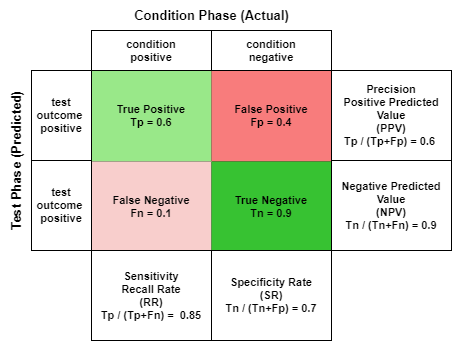
\includegraphics[width=0.9\textwidth]{DrawIo/ConfusionMatrixMotDet.png}
    \end{figure}


    \subsubsection{Object Detection}
    Il secondo metodo testato per la sorveglianza è l'object detection. Sono state confrontate 4 reti neurali per trovare la più adatta tra prestazioni e precisione. Nonostante sia stata scelta la board Raspberry tenendo il considerazione la potenza di calcolo, i fotogrammi al secondo hanno subito una brusca riduzione rispetto alla soluzione precedente. Il parametro minimo è stato fissato a 1 FPS, sotto il quale il divario temporale tra due immagini analizzate mancherebbe la rilevazione di possibili avvenimenti. La causa principale di tale crollo nelle prestazioni utilizzando questa soluzione è la mancanza di una GPU adatta nei Raspberry. Tale carenza è comunque colmabile con l'acquisto di espansioni USB dedicate all'espansione delle capacità grafiche della board (TPU).
    Immediatamente è risultato palese che le architetture delle reti tradizionalmente usate sui pc fossero troppo pesanti per il sistema ospitante. Per referenza è stata lasciata l'architettura (già di per se performante) Yolo3. Il focus quindi è stato soprattutto sull'individuazione di reti "leggere" che offrissero prestazioni adeguate. Sono state confrontate e testate le varie versioni "Tiny" della stessa rete come in tabella seguente:
        
    \begin{figure}[H]
        \centering
        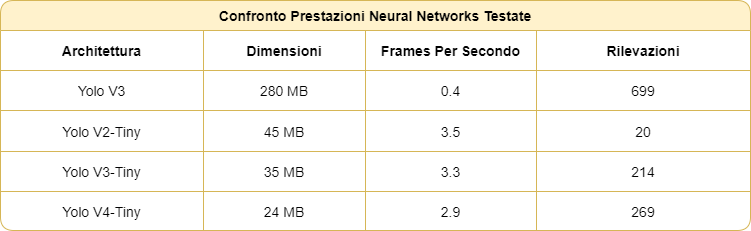
\includegraphics[width=0.9\textwidth]{DrawIo/ConfrontoNeuralNetworks.png}
    \end{figure}
    
    Dopo l'analisi è risultato chiara la scelta della versione Yolo V4-Tiny, con il miglior numero di rilevazioni e una velocità adeguata alla videosorveglianza.
    
    \begin{figure}[H]
        \caption{Surveillance with Object Detection}
        \label{fig:ODcomparison}
        \centering
        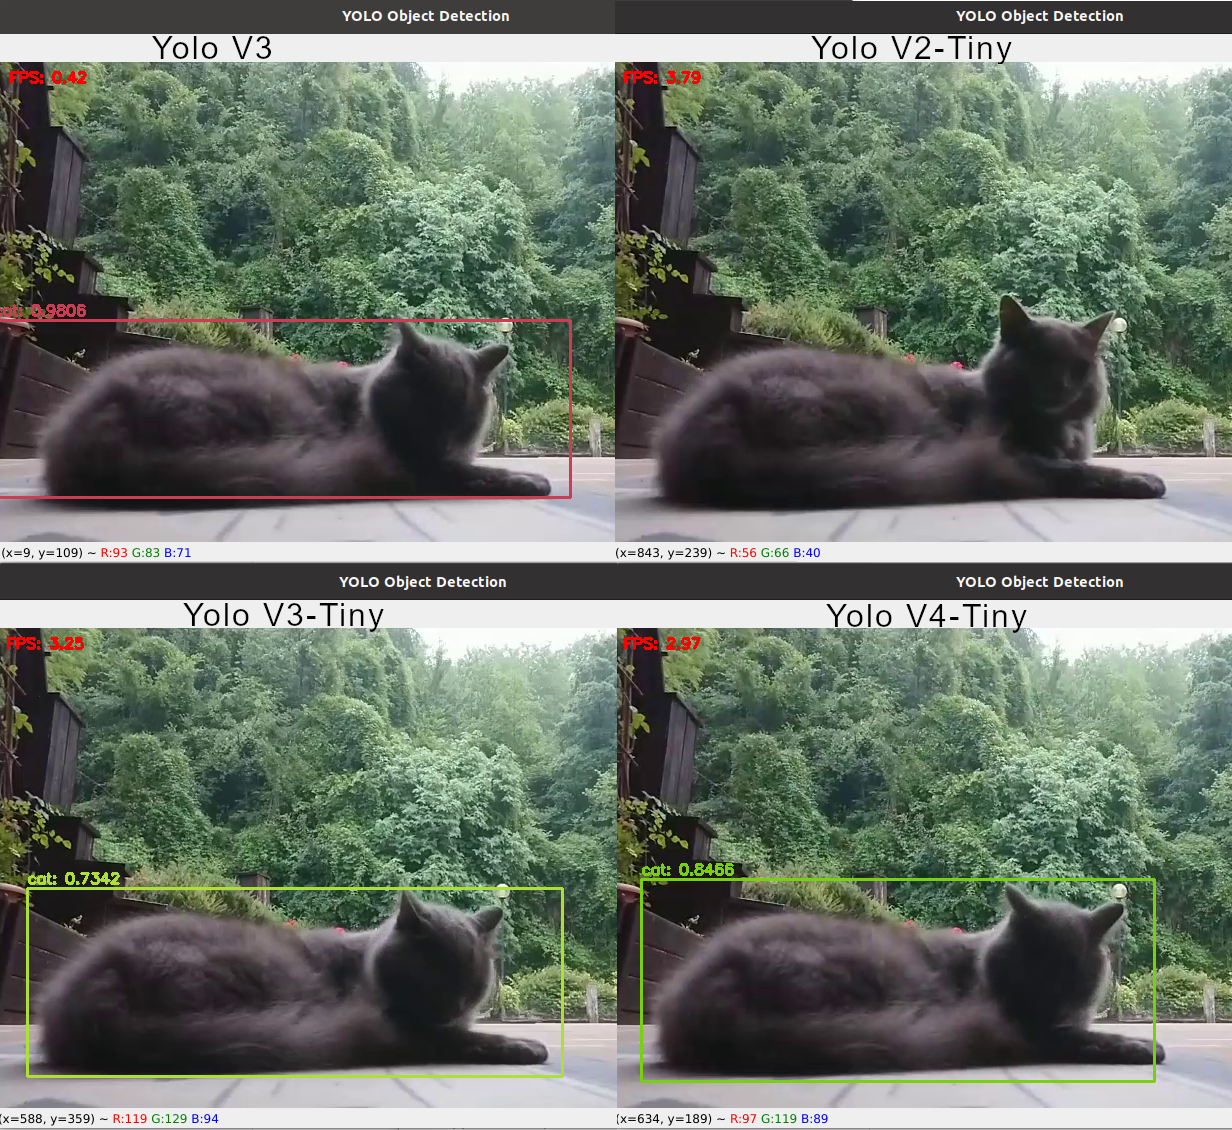
\includegraphics[width=1\textwidth]{Images/ODcomparison.png}
    \end{figure}
    
    Le prestazioni sono state a livello di precisione sono state alte, come ci si aspetta da una rete neurale comparata "in the wild" a metodi tradizionali. Di seguito si riporta la matrice di confusione delle prove effettuate:
    
    \begin{figure}[H]
        \caption{Confusion matrix of Object Detection}
        \label{fig:ODmatrix}
        \centering
        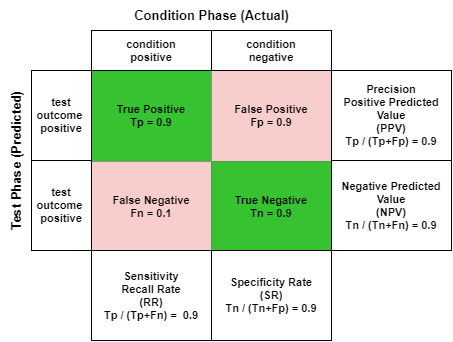
\includegraphics[width=0.9\textwidth]{DrawIo/ConfusionMatrixObjDet.png}
    \end{figure}